\documentclass[type=bachelor]{thuthesis}
% 选项:
%   type=[bachelor|master|doctor|postdoctor], % 必选
%   secret,                                   % 可选
%   pifootnote,                               % 可选(建议打开)
%   openany|openright,                        % 可选,基本不用
%   arial,                                    % 可选,基本不用
%   arialtoc,                                 % 可选,基本不用
%   arialtitle                                % 可选,基本不用

% 所有其它可能用到的包都统一放到这里了,可以根据自己的实际添加或者删除。
\usepackage{thuthesis}

% 定义所有的图片文件在 figures 子目录下
\graphicspath{{figures/}}

% 可以在这里修改配置文件中的定义。导言区可以使用中文。
% \def\myname{薛瑞尼}

\begin{document}

%%% 封面部分
\frontmatter
\thusetup{
  %******************************
  % 注意:
  %   1. 配置里面不要出现空行
  %   2. 不需要的配置信息可以删除
  %******************************
  %
  %=====
  % 秘级
  %=====
  secretlevel={秘密},
  secretyear={10},
  %
  %=========
  % 中文信息
  %=========
  ctitle={虚拟容器管理系统设计与实现},
  cdegree={工学学士},
  cdepartment={计算机科学与技术系},
  cmajor={计算机科学与技术},
  cauthor={陈天昱},
  csupervisor={姜进磊副教授},
  % 日期自动使用当前时间,若需指定按如下方式修改:
  % cdate={超新星纪元},
  %
  % 博士后专有部分
  cfirstdiscipline={计算机科学与技术},
  cseconddiscipline={系统结构},
  postdoctordate={2009年7月——2011年7月},
  id={编号}, % 可以留空: id={},
  udc={UDC}, % 可以留空
  catalognumber={分类号}, % 可以留空
  %
  %=========
  % 英文信息
  %=========
  etitle={The Design and Implementation of a Linux Container Management System},
  % 这块比较复杂,需要分情况讨论:
  % 1. 学术型硕士
  %    edegree:必须为Master of Arts或Master of Science(注意大小写)
  %             “哲学、文学、历史学、法学、教育学、艺术学门类,公共管理学科
  %              填写Master of Arts,其它填写Master of Science”
  %    emajor:“获得一级学科授权的学科填写一级学科名称,其它填写二级学科名称”
  % 2. 专业型硕士
  %    edegree:“填写专业学位英文名称全称”
  %    emajor:“工程硕士填写工程领域,其它专业学位不填写此项”
  % 3. 学术型博士
  %    edegree:Doctor of Philosophy(注意大小写)
  %    emajor:“获得一级学科授权的学科填写一级学科名称,其它填写二级学科名称”
  % 4. 专业型博士
  %    edegree:“填写专业学位英文名称全称”
  %    emajor:不填写此项
  edegree={Bachelor of Engineering},
  emajor={Computer Science and Technology},
  eauthor={CHEN Tianyu},
  esupervisor={Associate Professor JIANG Jinlei},
  % 日期自动生成,若需指定按如下方式修改:
  % edate={December, 2005}
  %
  % 关键词用“英文逗号”分割
  ckeywords={虚拟化, 虚拟容器, 分布式系统, 性能测试, 应用自动部署},
  ekeywords={Virtualization, Linux Container, Distributed Systems, Benchmark, Application Automatic Deployment}
}

% 定义中英文摘要和关键字
\begin{cabstract}
  论文的摘要是对论文研究内容和成果的高度概括。摘要应对论文所研究的问题及其研究目
  的进行描述,对研究方法和过程进行简单介绍,对研究成果和所得结论进行概括。摘要应
  具有独立性和自明性,其内容应包含与论文全文同等量的主要信息。使读者即使不阅读全
  文,通过摘要就能了解论文的总体内容和主要成果。

  论文摘要的书写应力求精确、简明。切忌写成对论文书写内容进行提要的形式,尤其要避
  免“第 1 章……;第 2 章……;……”这种或类似的陈述方式。

  本文介绍清华大学论文模板 \thuthesis{} 的使用方法。本模板符合学校的本科、硕士、
  博士论文格式要求。

  本文的创新点主要有:
  \begin{itemize}
    \item 用例子来解释模板的使用方法;
    \item 用废话来填充无关紧要的部分;
    \item 一边学习摸索一边编写新代码。
  \end{itemize}

  关键词是为了文献标引工作、用以表示全文主要内容信息的单词或术语。关键词不超过 5
  个,每个关键词中间用分号分隔。(模板作者注:关键词分隔符不用考虑,模板会自动处
  理。英文关键词同理。)
\end{cabstract}

% 如果习惯关键字跟在摘要文字后面,可以用直接命令来设置,如下:
% \ckeywords{\TeX, \LaTeX, CJK, 模板, 论文}

\begin{eabstract}
   An abstract of a dissertation is a summary and extraction of research work
   and contributions. Included in an abstract should be description of research
   topic and research objective, brief introduction to methodology and research
   process, and summarization of conclusion and contributions of the
   research. An abstract should be characterized by independence and clarity and
   carry identical information with the dissertation. It should be such that the
   general idea and major contributions of the dissertation are conveyed without
   reading the dissertation.

   An abstract should be concise and to the point. It is a misunderstanding to
   make an abstract an outline of the dissertation and words ``the first
   chapter'', ``the second chapter'' and the like should be avoided in the
   abstract.

   Key words are terms used in a dissertation for indexing, reflecting core
   information of the dissertation. An abstract may contain a maximum of 5 key
   words, with semi-colons used in between to separate one another.
\end{eabstract}

% \ekeywords{\TeX, \LaTeX, CJK, template, thesis}

% 如果使用授权说明扫描页,将可选参数中指定为扫描得到的 PDF 文件名,例如:
% \makecover[scan-auth.pdf]
\makecover

%% 目录
\tableofcontents

%% 符号对照表
\begin{denotation}[3cm]
\item[LXC] 虚拟容器 (Linux Container)
\item[time-sharing] 分时
\item[AWS] 亚马逊云计算服务 (Amazon Web Services)
\item[IaaS] 基础设施服务 (Infrastructure as a Service)
\item[PaaS] 平台服务 (Platform as a Service)
\item[SaaS] 软件服务 (Software as a Service)
\item[hypervisor] 虚拟机管理程序
\item[instance] 虚拟机实例
\item[LAN] 局域网 (Local Area Network)
\item[VLAN] 虚拟局域网 (Virtual Local Area Network)
\item[SAN] 存储区域网络 (Storage Area Network)
\item[NAS] 网络附属存储 (Network Attached Storage)
\item[Object Storage] 对象存储
\item[Block Storage] 块存储
\end{denotation}



%%% 正文部分
\mainmatter
\chapter{引言}
\label{cha:intro}

\section{选题背景}

\subsection{云计算的历程}

云计算的概念诞生的远远比它的名字更早。它的概念可以追溯到早期的
分时系统\footnote{time-sharing systems}。

早期的计算机系统价格昂贵,而且体积庞大,使得个人用户很难拥有独立的个人计算机 (PC) 。
这就导致了多个用户可以同时使用同一个计算资源——例如一台电子计算机——的分时系统
~\cite{timesharing}的产生。所谓分时系统,就是有一个主要的
计算系统 (mainframe computer) ,用户通过终端机 (terminal) 连接到这个
系统上使用计算资源。用户一般而言不需要考虑计算机操作系统乃至硬件的具体细节——因为自然
有管理员管理这些细节,只需要像“租客”一样使用计算资源就可以了。现代的操作系统,
例如 GNU/Linux 或者 Microsoft Windows ,都支持多用户模式。

\begin{figure}[h]
    \centering
    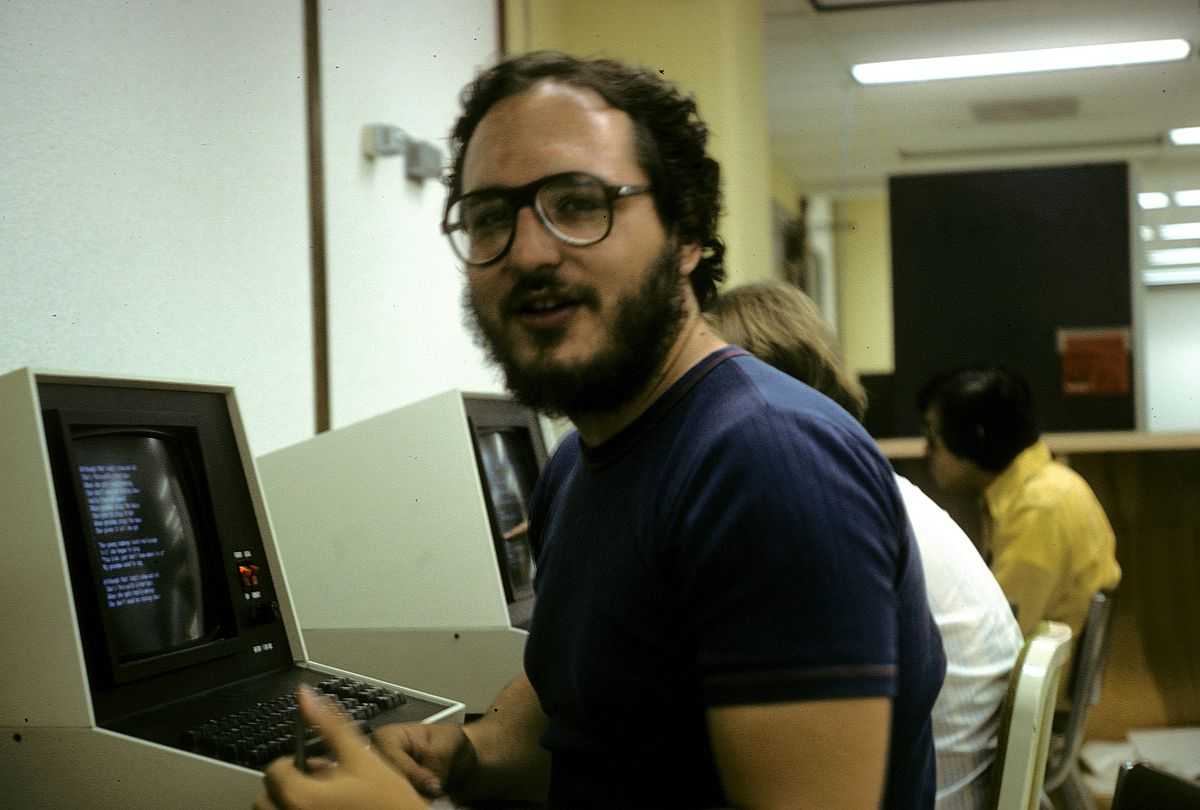
\includegraphics[height=0.5\textwidth]{unix_time_sharing}
    \caption{威斯康辛大学麦迪逊分校的学生使用终端机,1978 年}
\end{figure}

从 2000 年左右开始,云计算的概念正式形成了。2006 年诞生的 Amazon EC2 \footnote{EC2
  是 Elastic Compute Cloud 的缩写,因有两个连着的 C 所以叫做 EC2 ,不是
  “第二个版本”的意思。}成为了迄今最成功的云计算平台之一。2008 年诞生的 OpenNebula
是另一个云计算平台,顾名思义它是一个自由软件\footnote{Free as in freedom}
,使用 Apache License 发布。

而现在更加流行的自由的云计算平台是 OpenStack 。OpenStack 最初是由
 NASA 和 RackSpace 共同发起的,从 2012 年开始由叫做 OpenStack Foundation 的非营利
组织进行开发和维护。它和 Amazon EC2 的最大不同就是它是完全自由和开源的。不但可以利用
这个软件搭建自己的云计算环境,而且可以对相关的代码展开研究。OpenStack 中的主要组成部分
和 Amazon AWS 中的部分具有一定的对应关系,比如 AWS 的核心也就是 EC2 对应了 OpenStack
 里的 Nova ,负责虚拟机的调度和管理;AWS 中的简单存储模块 S3 在 OpenStack 中
有 Swift 与之对应~\cite{openstack}。

\subsection{云计算平台的服务类型}

云计算提倡的概念是“所有都是服务”
 (everything as a service) ~\cite{cloud-and-openstack},也就是用户不直接接触
物理上的计算机,但是却能通过网络获得相应的计算服务。云计算的“云”不在本地,这就好比大家
每天日常生活都要使用电,但极少有人在家里自己搭建一台柴油发电机,而是在发电厂集中发电,
然后通过输电线路把电力输送到千家万户供人们使用。数据中心就好像这个发电厂,计算机网络
就好像电线,终端用户就像使用电力一样使用云计算产生的计算资源。

根据服务类型不同,云计算平台主要可以分为以下三种——基础设施
服务 (IaaS)、平台服务 (PaaS) 还有软件服务 (SaaS) ~\cite{types-of-cloud}。

\subsubsection{基础设施服务}

顾名思义,这种服务类型就是只提供必要的设施,而不提供上层应用。这些设施包括由虚拟机管理程序
支持的大量的虚拟机集群、操作系统磁盘镜像存储池(这样用户在创建虚拟机实例的时候就不用联网
从镜像源下载镜像,直接从镜像存储服务调取相应的镜像即可)、文件存储服务、防火墙、负载均衡器
等等。

当然还有虚拟局域网。例如某大学计算机系有网络和操作系统两个实验室,它们共享一套虚拟机集群。
网络实验室和操作系统实验室希望各占用一个子网。如果是使用物理上的局域网,那么应该有两个交换机,
各接入路由器的两个物理端口上。而使用了虚拟局域网,就可以用两个逻辑端口代替。使用虚拟局域网,
可以缩小广播域,从而提高集群的安全性。

上文提到的 Amazon EC2 就是一个典型的 IaaS 平台。类似的,OpenStack 也是一个 IaaS 平台,
截至到 2016 年,一共包含以下几个核心组成部分~\cite{openstack}:

\begin{enumerate}
    \item \textbf{Nova:} Nova 是 OpenStack 的计算部分,主要负责虚拟机管理。它的 API
    可以和 Amazon EC2 的相兼容,RackSpace 的商业计算服务就是建立在 Nova 上的。
    \begin{enumerate}
        \item \textbf{nova-compute}
        \item \textbf{nova-scheduler}
        \item \textbf{nova-conductor}
        \item \textbf{nova-db}
        \item \textbf{nova-console}
        \item \textbf{nova-cert}
        \item \textbf{nova-objectstore}
    \end{enumerate}
    \item \textbf{Neutron:}
    \item \textbf{Swift:}
    \item \textbf{Cinder:}
    \item \textbf{Keystone:}
    \item \textbf{Glance:}
\end{enumerate}


\subsubsection{平台服务}

\subsubsection{软件服务}

\subsection{虚拟化和云计算}

\section{研究价值和主要贡献}

\section{论文结构}

